\section{Characterization of the FBG-based FOS}
The main efforts were concentrated to optimize the design of the polyimide-coated FBG sensors in order to be able to measure in low temperatures. Yeo et al.~\cite{YEO_PI} found out that \gls{RH} sensitivity increases linearly with coating thickness, but the time response increases as well (see figure~\ref{fig:yeo}). The \gls{RH} sensitivity increases linearly with the coating thickness, so in principle, a better humidity sensitivity would result in a more precise sensor.

\begin{figure}[!h]
\centering
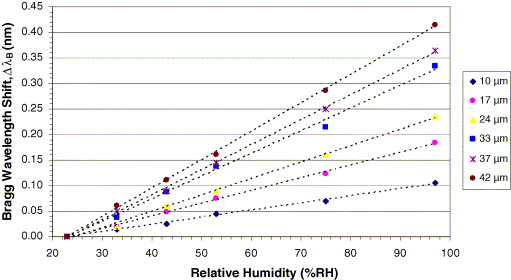
\includegraphics[width=0.80\columnwidth]{Chapter5/images/yeo_coating.jpg}
\caption{RH response of the sensors with different coating thicknesses, from 23 to 97\%RH at constant room temperature~\cite{YEO_PI}.}
\label{fig:yeo}
\end{figure}

The higher thickness increases time response, as seen in Figure~\ref{fig:yeo2}. The most dangerous scenarios in \gls{STS} include an uncontrolled change of humidity, which should be detected within minutes to conduct necessary actions in the control system. Therefore, the chosen coating thickness is between \SI{15}{\micro\metre} and \SI{20}{\micro\metre}, slightly higher than the first reported distributed sensing system implemented for the \gls{CMS} at \gls{CERN}, where \SI{10}{\micro\metre} were used. 
\begin{figure}[!h]
\centering
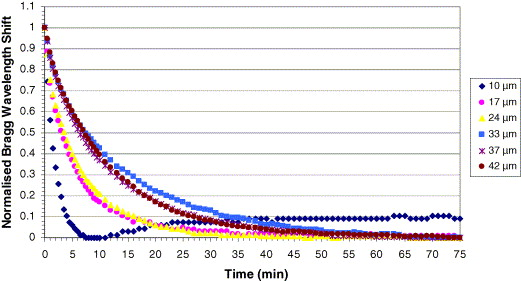
\includegraphics[width=0.80\columnwidth]{Chapter5/images/time_response_yeo.jpg}
\caption{Recovery time of the sensors from 75 to 33\% RH~\cite{YEO_PI}.}
\label{fig:yeo2}
\end{figure}
\newpage
Two different \gls{FOS} designs were compared:
\begin{itemize}
    \item a multiplexed version with 5 \glspl{FBG} inscribed in a germanium-doped fiber (see figure~\ref{fig_array_photo}). The polyimide layer was applied in four steps, \SI{5}{\micro\metre} each with \SI{1.25}{\micro\metre} uncertainty for each layer. In total, the coating thickness was about \SI{20}{\micro\metre}$\pm$\SI{5}{\micro\metre}. The temperature compensation was ensured by a second \gls{FBG} array which measures only temperature,
    \item the second design is a hygrometer with temperature and humidity sensors inscribed into one fiber. The coating thickness was chosen to be \SI{15}{\micro\metre}. The tested sensors are depicted in Figure~\ref{fig_single_photo}.
\end{itemize}

\begin{figure}[!h]
\centering
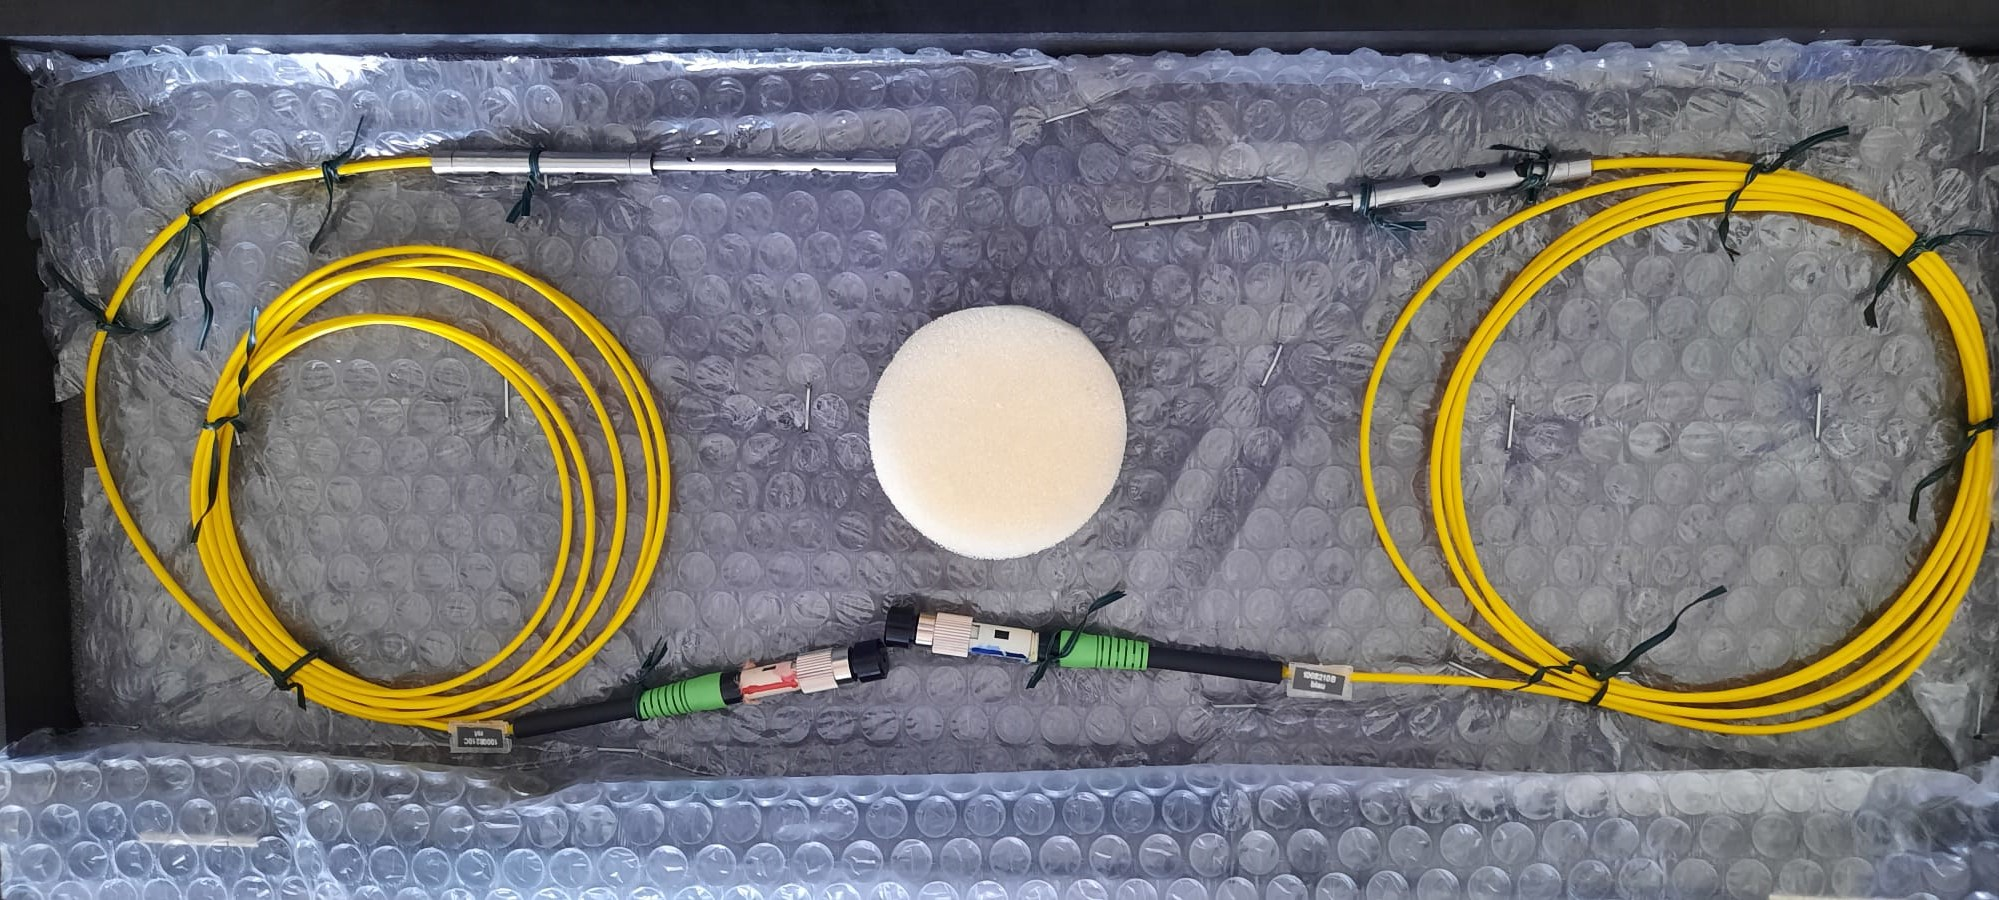
\includegraphics[width=0.7\columnwidth]{Chapter5/images/single1.jpeg}
\caption{Hygrometer (temperature and humidity sensitive \glspl{FBG} inscribed into the same fiber). The only difference between the two hygrometers in the photo is the diameter of the holder/packaging of the \gls{RH} sensitive \gls{FBG} (manufactured by AOS GmbH~\cite{AOS}).}
\label{fig_single_photo}
\end{figure}

\begin{figure}[!h]
\centering
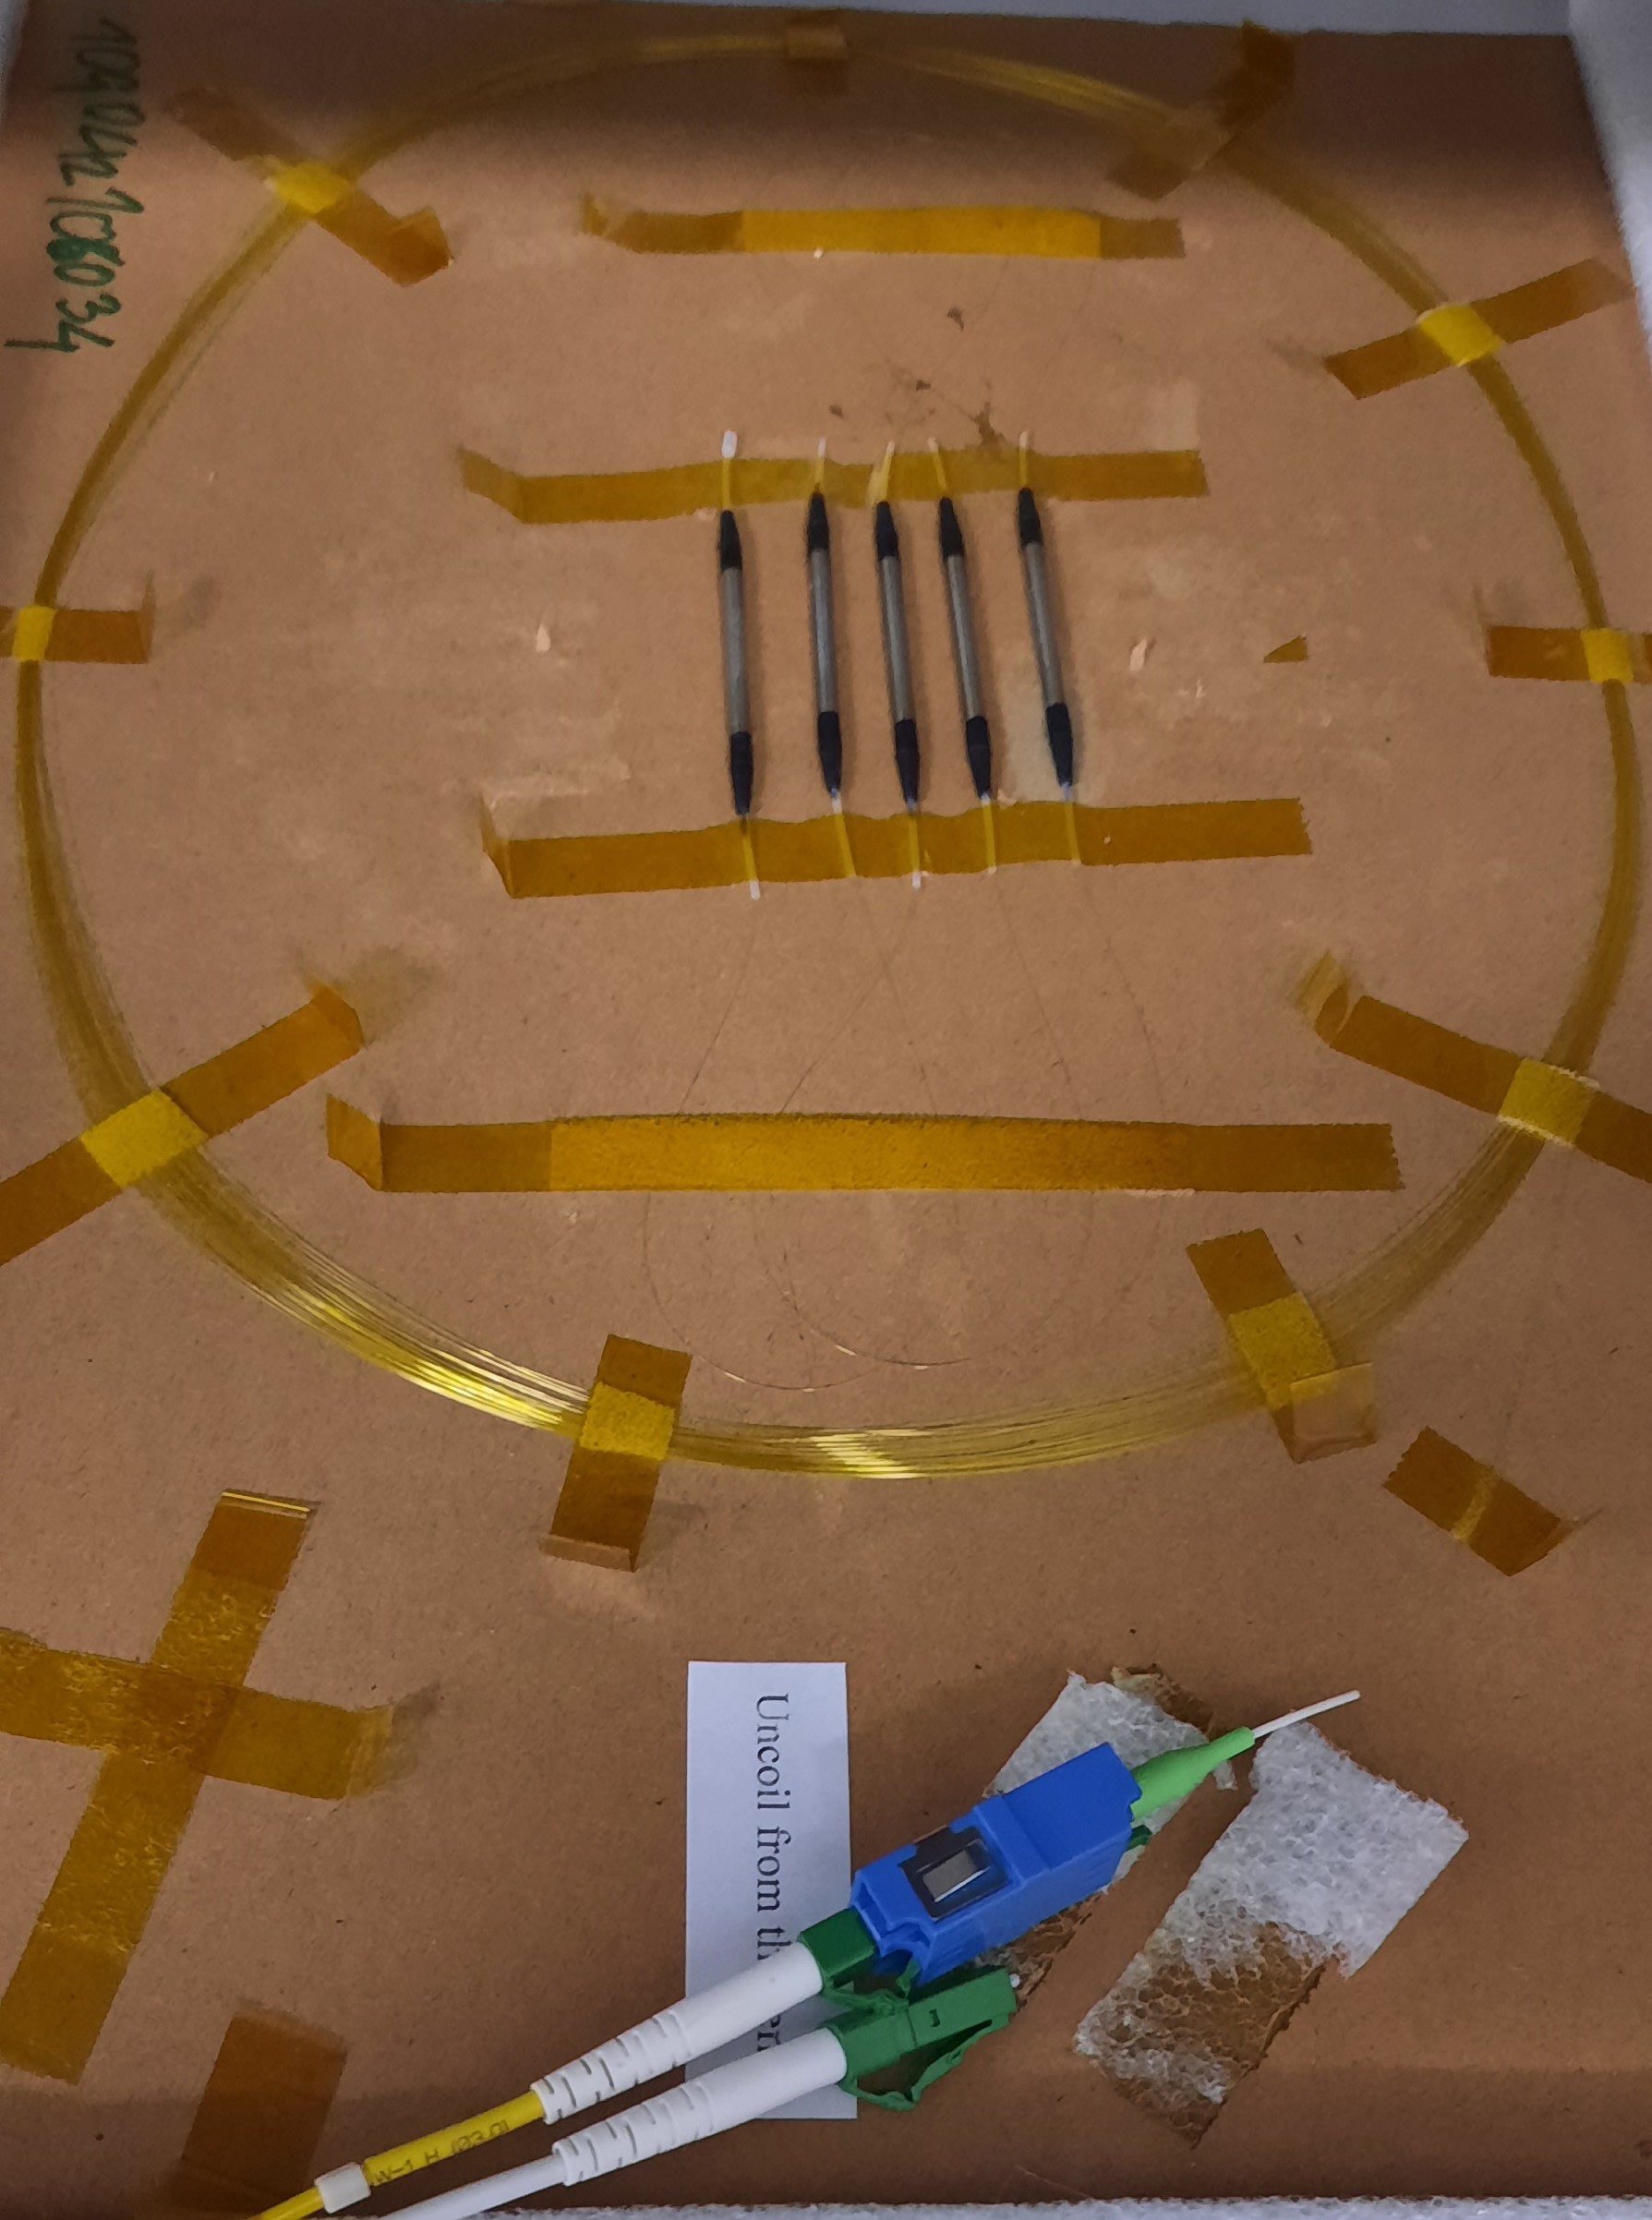
\includegraphics[angle=90,width=0.43\columnwidth]{Chapter5/images/t_array1.jpg}
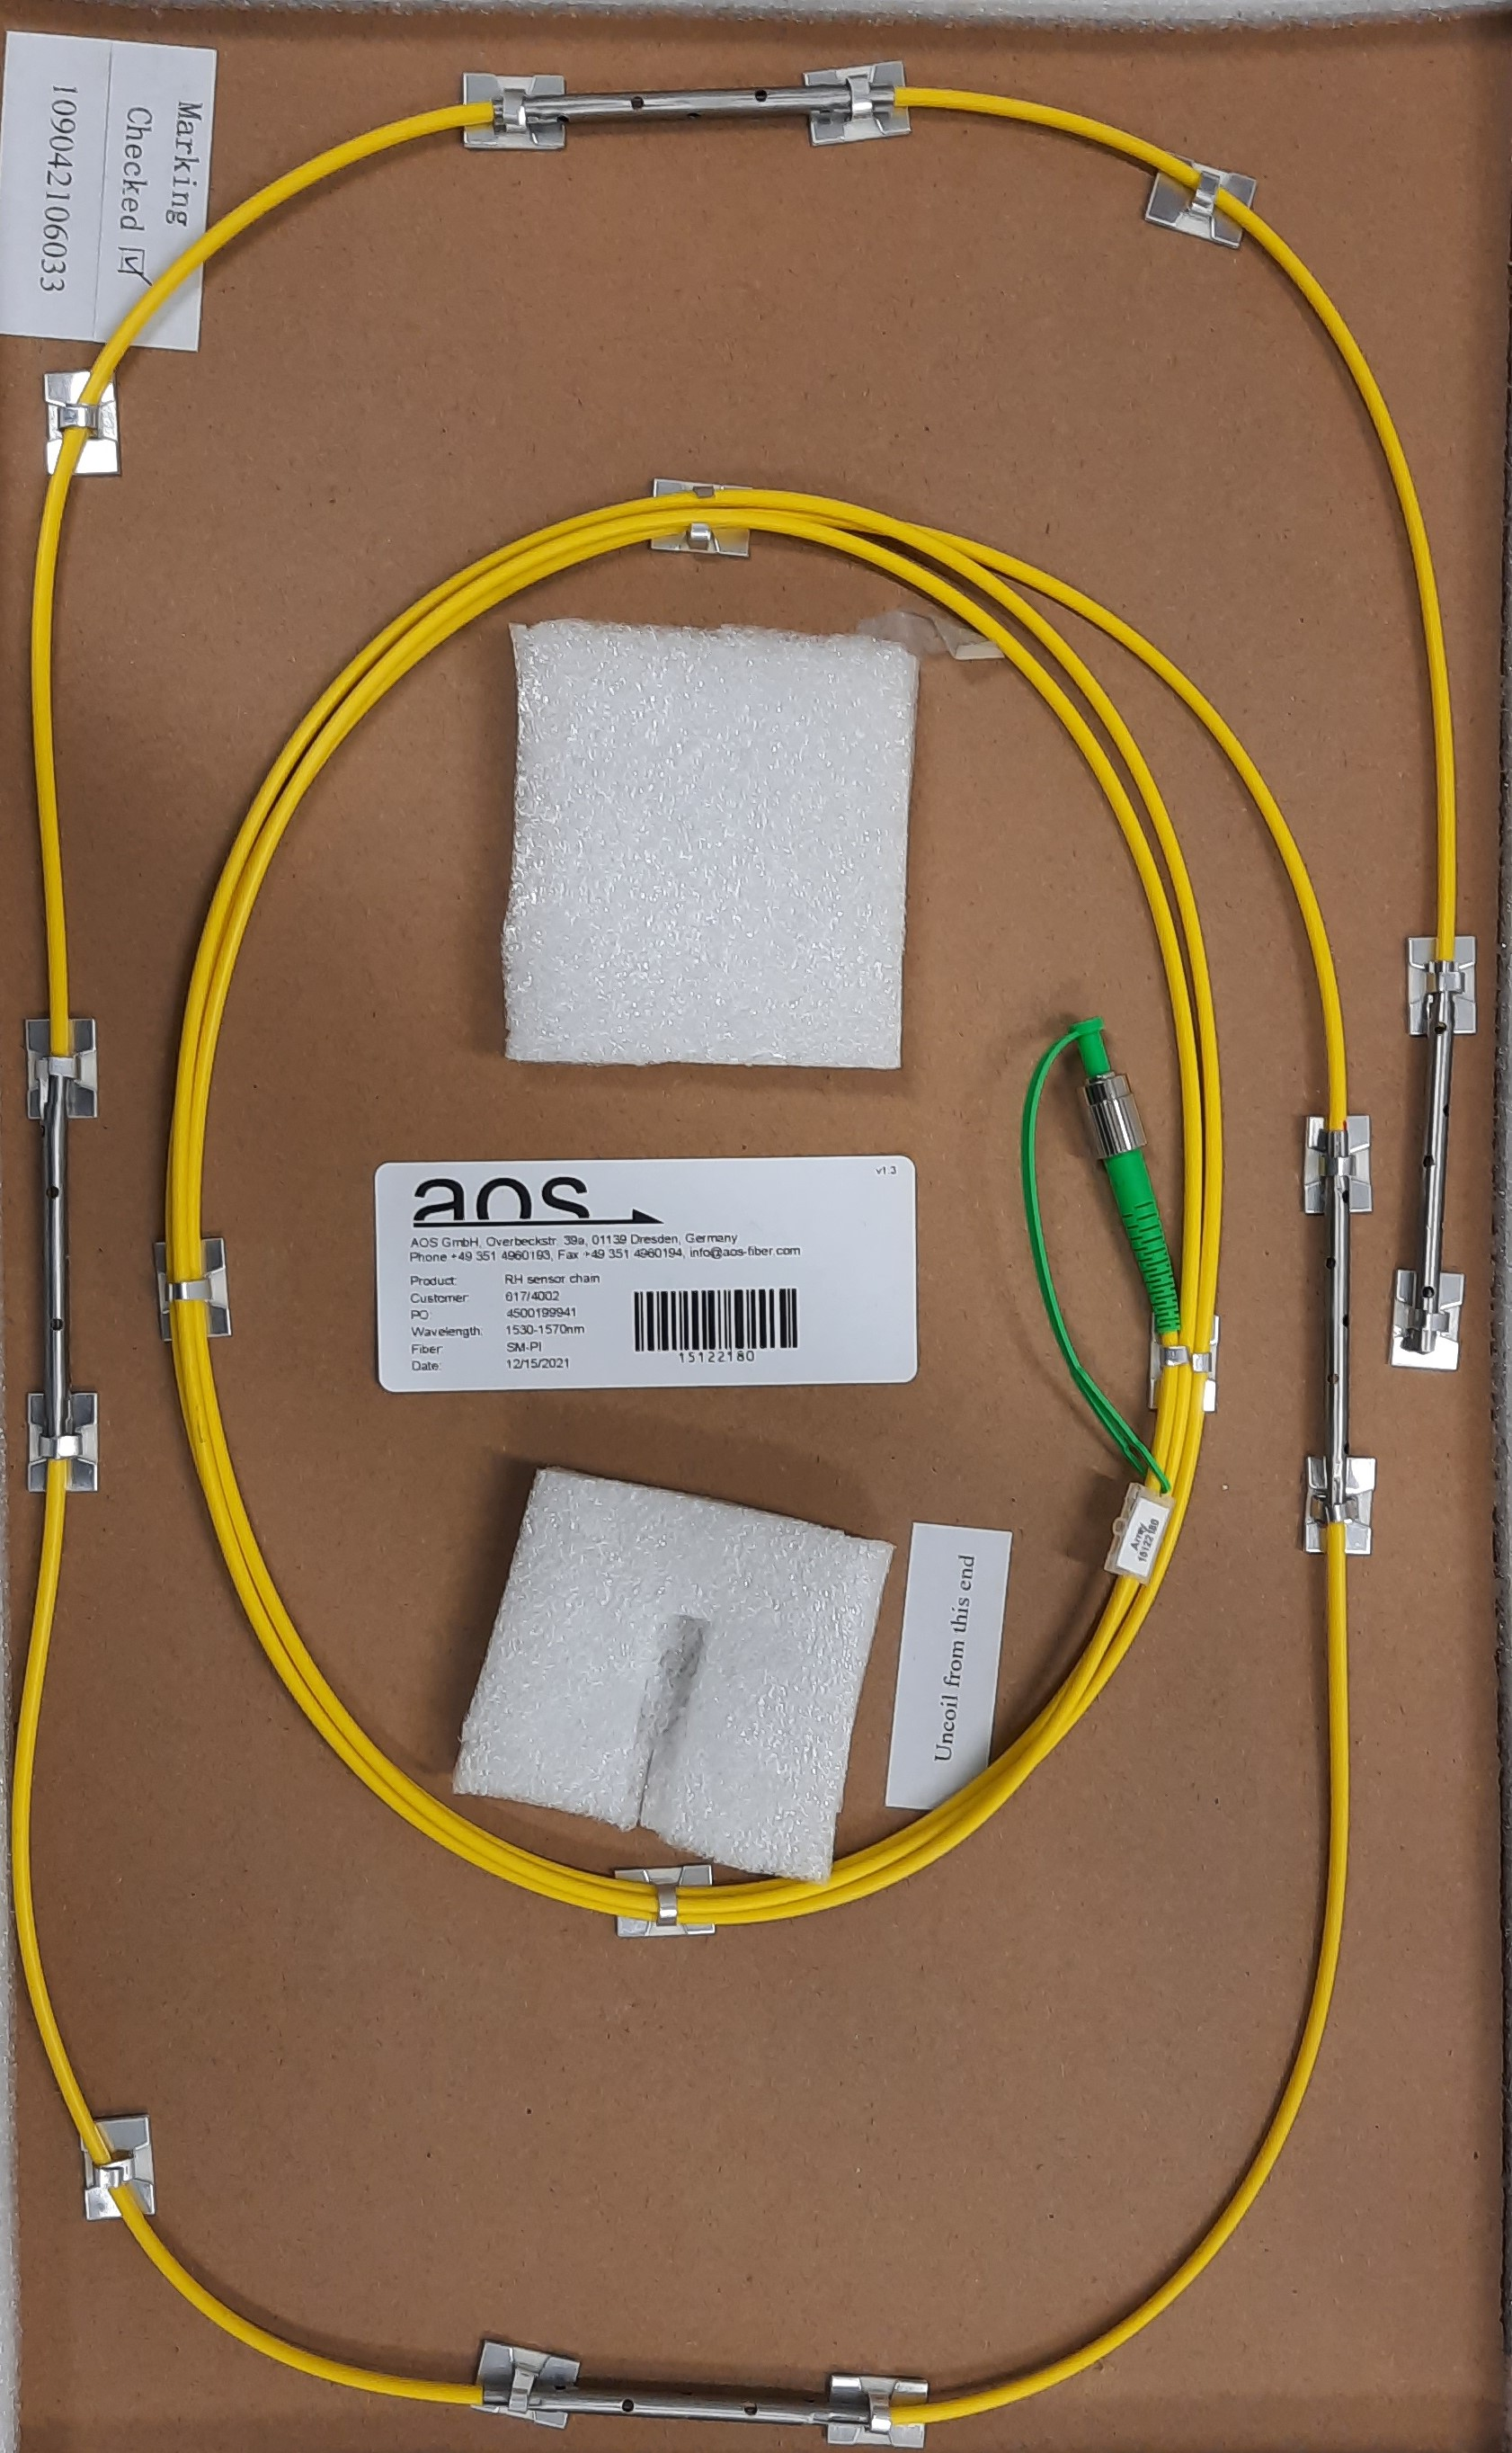
\includegraphics[angle=90,width=0.52\columnwidth]{Chapter5/images/rh_array1.jpg}
\caption{The left photo shows the temperature sensing array, and the right one shows the \gls{RH} sensing array after packaging the FBG in strain-free conditions. The fibers do not have the jacket applied on the polyimide coating. The arrays were manufactured by Technica~\cite{technica} and packaged by AOS Electronics~\cite{AOS}.}
\label{fig_array_photo}
\end{figure}
To characterize a RH FBG-based sensor, the humidity, and temperature sensitivity coefficient have to be determined. In addition to that, parameters like time response, hysteresis, or repeatability contribute to the total uncertainty of the sensor. 
\section{Experimental setup}
\label{fos:setup}

The sensors were calibrated using a S8000 chilled mirror hygrometer~\cite{michell_s8000}. Additionally, to compare the results, two industrial \gls{RH} sensors were used: HYT221 and SHT85 (see section \ref{capacitive_sensors}). The temperature during the testing was controlled by a Binder MKF chamber~\cite{binder} which offers also relative humidity control down to \SI{0}{\celsius}. The experimental setup scheme is shown in Figure~\ref{fig:fos_arch}. 

Two calibration methods were used to characterize the \gls{FBG}-based relative humidity sensors. The first method involved the use of different saturated salt solutions:
\begin{itemize}
    \item lithium chloride - \gls{RH} at \SI{25}{\celsius} 11\%
    \item magnesium(II) chloride - \gls{RH} at \SI{25}{\celsius} 33\%
    \item sodium chloride - \gls{RH} at \SI{25}{\celsius} 75\%
\end{itemize}
 Saturated salt solutions have well-defined relative humidity values at a given temperature~\cite{Fossa:687857}. This method offers a cost-effective way to calibrate a \gls{RH}. The second method relied on the humidity control (10\% to 80\% with a 10\% increment) of the climatic chamber.
 
 The sensing instrument (light source) was the Micron Optics Hyperion SI255~\cite{si255}. The SI255 is supplied with high power, low noise, ultra-wide swept wavelength laser. It is guaranteed to provide absolute accuracy of 1~pm at every scan within the operating range of 1500 -- 1600~nm~\cite{si255}.

The setup was controlled by the developed \gls{EPICS} based framework. The custom-written \glspl{IOC} were used to obtain data from the temperature and humidity sensors, as well as from the climatic chamber. The data related to the fiber optic sensors were collected through ENLIGHT\footnote{ENLIGHT Sensing Analysis Software is a powerful utility that is included with Micron
Optics sensing interrogators.} software, and a custom \gls{IOC} connected to it. Subsequently, all the data was stored using an archiver appliance to a Redis database. 

\begin{figure}[!h]
\centering
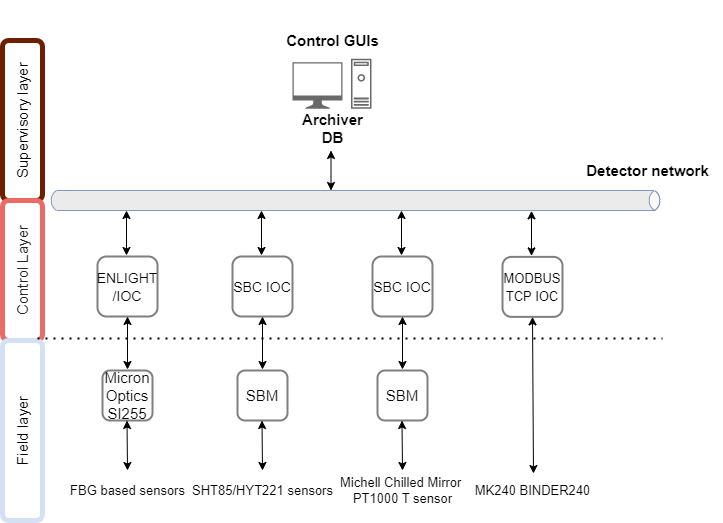
\includegraphics[width=0.85\columnwidth]{Chapter5/images/FOS_dcs_scheme.png}
\caption{Controls architecture for the temperature and humidity sensor measurement.}
\label{fig:fos_arch}
\end{figure}
\newpage
\subsection{Sensors characterization}

%To characterize the sensors and estimate their uncertainty, it's necessary to know the wavelength reflected at the \gls{FBG}. 
Initially, the basic parameters of the sensors were checked. The Bragg wavelength and the corresponding spectral response of the sensors. 
Figure~\ref{fig_hygrometer1} shows an example of the readout of the SI255 device from the hygrometer. In order to perform an accurate calibration of the sensors, the \gls{RH} and temperature sensitivity factors have to be determined.

The climatic chamber offers the temperature control between \SI{-40}{\celsius} and \SI{180}{\celsius}. As both methods to control humidity offer only limited capabilities, below \SI{0}{\celsius} for calibration of series production a new custom humidity control system will need to be considered~\cite{Berruti, Veldscholte:2021wjt}.
\begin{figure}[!h]
\centering
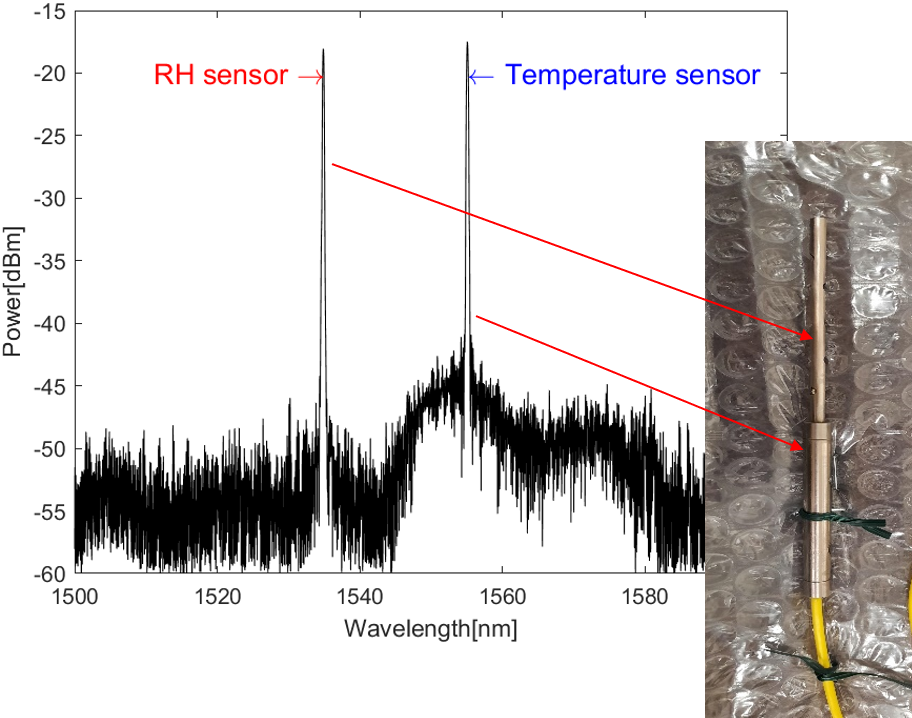
\includegraphics[width=0.6\columnwidth]{Chapter5/images/hygr.png}
\caption{The spectral response of the FBG reflected wavelength. Each of the peaks is correlated with one of the gratings in the fiber.}
\label{fig_hygrometer1}
\end{figure}
\newpage
One of the most important sensor characteristics is accuracy, which holds information about the deviation of the measured value from the ideal value. Overall, the uncertainty comprises several factors~\cite{sensors_physics}:
\begin{itemize}
    \item calibration error - a constant error over the whole range of measurements, its source is related to the accuracy of the reference device and the calibration method applied,
    \item hysteresis - a deviation of the sensor's output to a certain point of the input single when approached from opposite directions (see Figure~\ref{fig:accuracy}), 
    \item non-linearity - in the characterization of the \glspl{FBG} it is assumed that the response of the sensors to the stimulus (increasing humidity or temperature) is linear. Therefore, any deviation from the linearity is considered a contribution to the uncertainty,
    \item repeatability - the error caused by the inability of a sensor to represent the same value at the same conditions. 
\end{itemize}
\begin{figure}[!h]
\centering

\includegraphics[width=0.85\columnwidth]{Chapter5/images/Picture2.png}
\caption{Different contributions to the sensor's accuracy.}
\label{fig:accuracy}
\end{figure}
By combining all the errors, the total uncertainty of a sensor is as follows:
\begin{equation}
    \mu_{c} = \sqrt{\mu_{1}^{2} + \mu_{2}^{2} + ... + \mu_{i}^{2} + ... + \mu_{n}^{2}}
\end{equation}
The total uncertainty of a \gls{FBG} sensor may consist of many other factors (including the uncertainty of the peak wavelength measurement). Nevertheless, the factors listed above were considered to have the largest contribution. 

\section{Results}
\label{fbg_results}
In this section, the efforts to calibrate and characterize the humidity array and hygrometers are described in detail. The calibration relied on the Bragg wavelength shift measurements while increasing the \gls{RH} levels at the constant temperature value. This measurement was then repeated for different temperature values.
%It is a commonly used approach to estimate the humidity and temperature sensitivities~\cite{Berruti}. 

For the calibration with the saturated salt solutions, the sensors were exposed to the given salt for a prolonged time of about 6 hours. The calibration step in the climatic chamber lasted about 2 hours. Keeping the sensors for this time at constant conditions, ensured that the equilibrium was reached. 
\subsection{Characterization of RH FOS}

The test subjects were two hygrometers (\SI{15}{\micro\metre} polyimide coating) and  5 \gls{RH} sensors (\SI{20}{\micro\metre}) polyimide coating in an array with \SI{15}{\cm} distance between the subsequent sensors. The spectral response of the array can be in Figure~\ref{fig_array_wavelength}. The spectral responses are usually the first sign that the sensors perform correctly. 

\begin{figure}[!h]
\centering
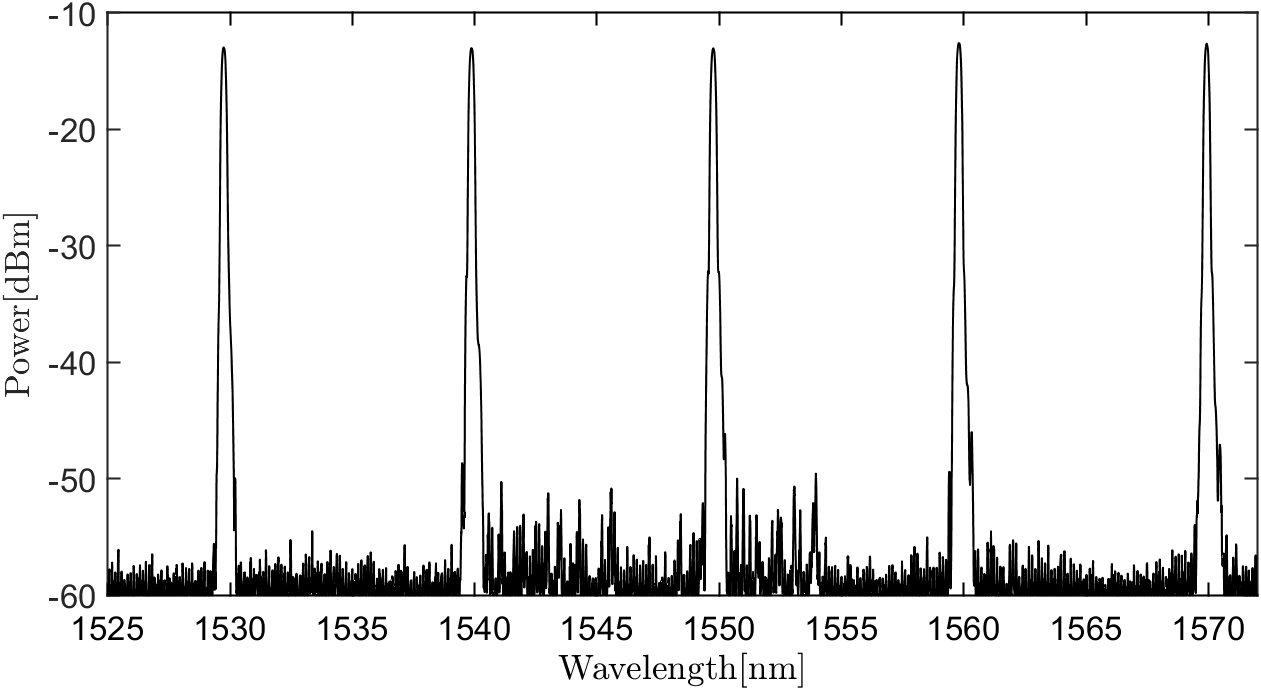
\includegraphics[width=0.85\columnwidth]{Chapter5/images/rh_array.png}
\caption{Spectral response of the RH sensors in the array.}
\label{fig_array_wavelength}
\end{figure}

The second test involved evaluating the humidity response of the sensor in the range (10\% to 80\%), see Figures~\ref{fig_response} and~\ref{fig_array_wavelength}. In both cases, increasing the relative humidity inside the test chamber results in the shift of the Bragg wavelength toward higher values. It's related to the increasing strain on the grating resulting from the deposition of water molecules in the polyimide. These measurements were taken at a stable temperature of \SI{20}{\celsius}.
\begin{figure}[!h]
\centering
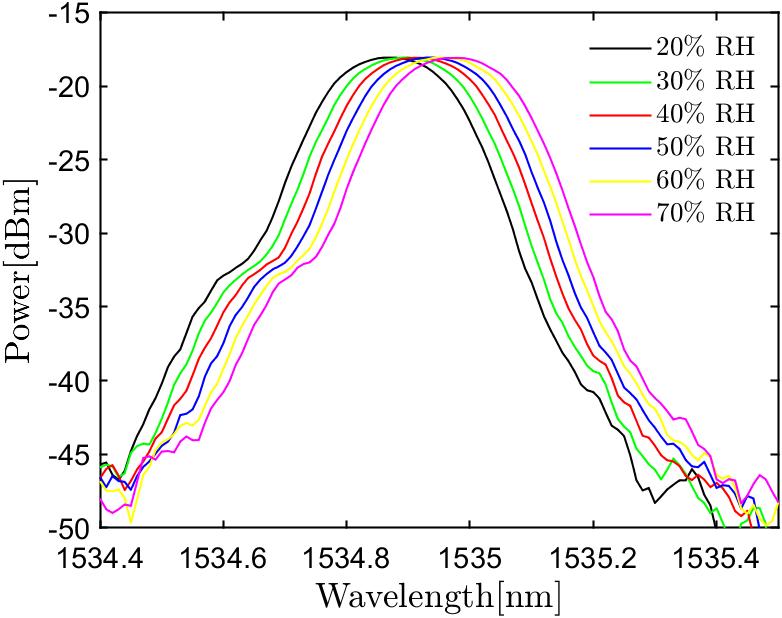
\includegraphics[width=0.45\columnwidth]{Chapter5/images/rh.png}
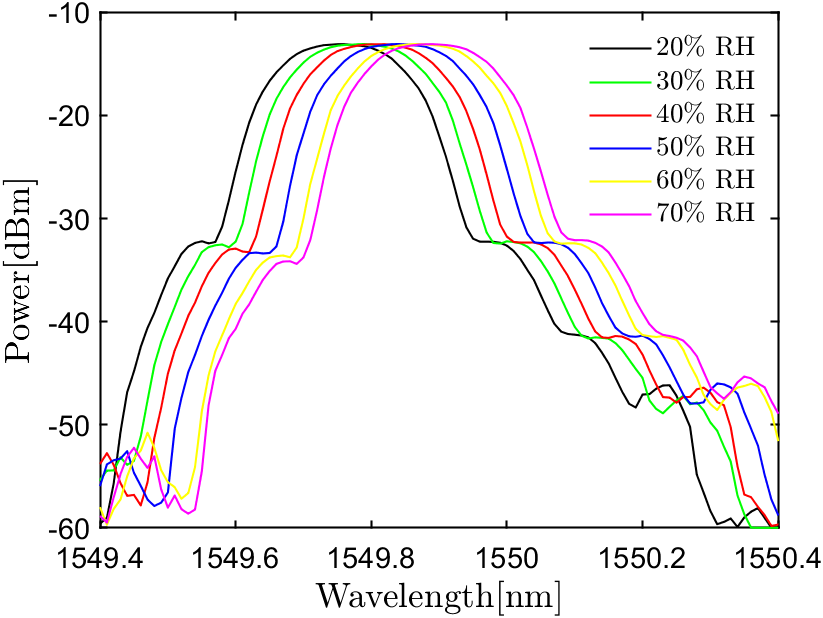
\includegraphics[width=0.475\columnwidth]{Chapter5/images/rh_array2.png}
\caption{Humidity induced Bragg wavelength shift of the hygrometer (left) and first sensor in the array (right). The spectral response is depicted as the power of the reflected wavelength. }
\label{fig_response}
\end{figure}
\newpage
Figures~\ref{fig_single_calibration} and~\ref{fig_array_calibration} depict the calibration curves of the hygrometer and one of the array sensors. The calibration curves were obtained by changing the humidity values from 10\% up to 80\% at a constant temperature. The temperature range was from \SI{-20}{\celsius} to \SI{30}{\celsius} with an increment of \SI{5}{\celsius}. Figures~\ref{fig_single_calibration} and~\ref{fig_array_calibration} depict a linear response to the humidity increase at every temperature.

The measurements below \SI{0}{\celsius} have relatively large uncertainty, due to the limited humidity control and fewer stable measurement points (due to humidity fluctuations). Furthermore, the change of temperature also results in the shift of the Bragg wavelength toward smaller values, which is also in agreement with results in~\cite{Kronenberg:02} and~\cite{Berruti}. In the array calibration, two curves for \SI{-5}{\celsius} and \SI{-10}{\celsius} are missing. This is related to the unrealistically high uncertainties, most likely caused by an additional strain applied to the sensors after handling. %The issue related to the array is discussed in the next sections.

\begin{figure}[!h]
\centering
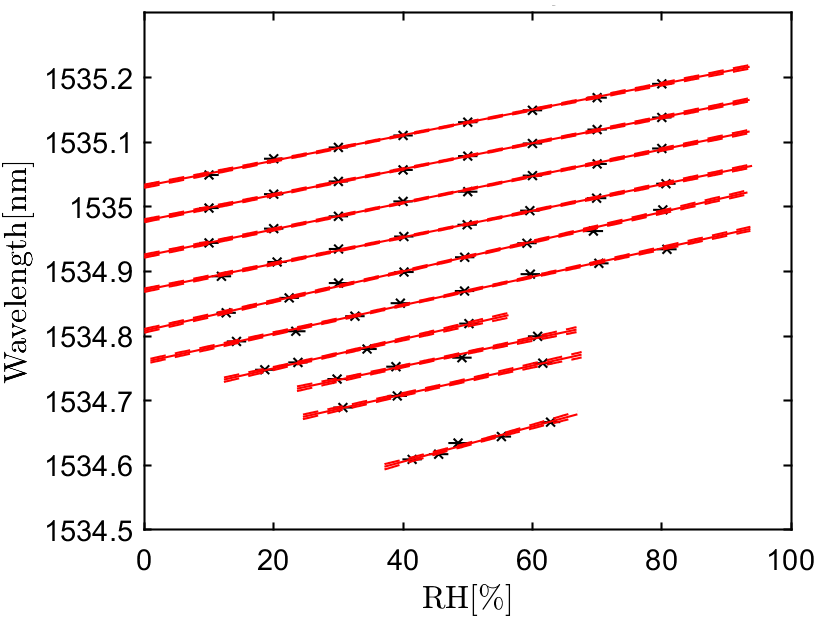
\includegraphics[width=0.67\columnwidth]{Chapter5/images/RHS.png}
\caption{Calibration curves for the hygrometer.}
\label{fig_single_calibration}
\end{figure}

\begin{figure}[!h]
\centering
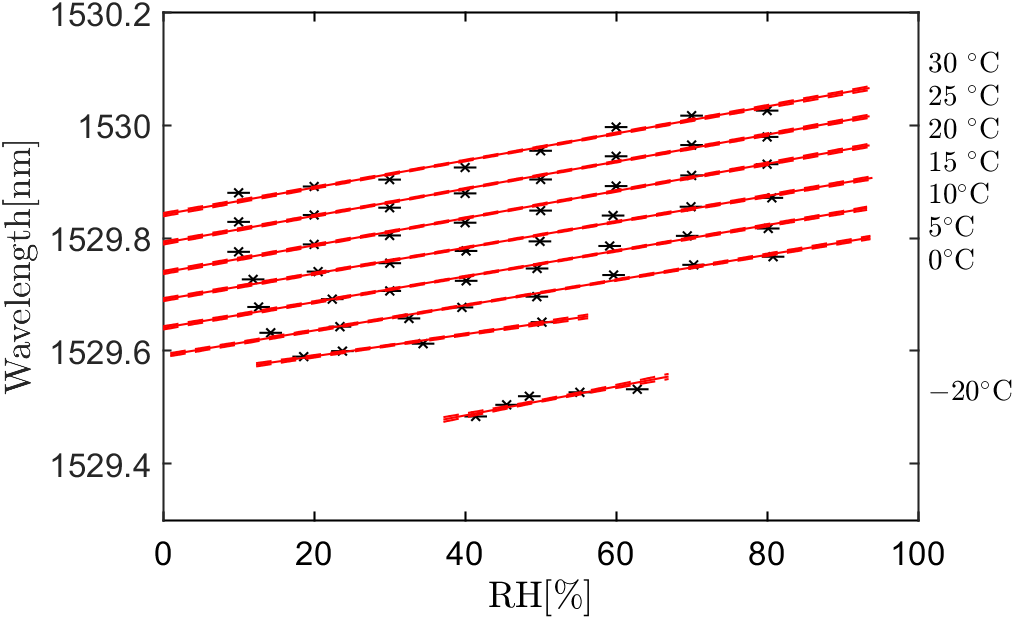
\includegraphics[width=0.67\columnwidth]{Chapter5/images/RH1.png}
\caption{Calibration curves for the first \gls{RH} sensor in the array.}
\label{fig_array_calibration}
\end{figure}
%\newpage
The uncertainties of the reference devices (the Michell chilled mirror $\pm 1$\%RH and the PT1000 temperature sensor's - \SI{0.001}{\celsius}) are taken into account, together with linear fit error. The uncertainties are assumed to be following the Gaussian distribution and the confidence level of 68\%. The slopes of the obtained fits are the humidity sensitivities of the sensors. These values at different temperatures and their corresponding uncertainties are depicted in Figure~\ref{fig_RH_sens}. 

\begin{figure}[!h]
\centering
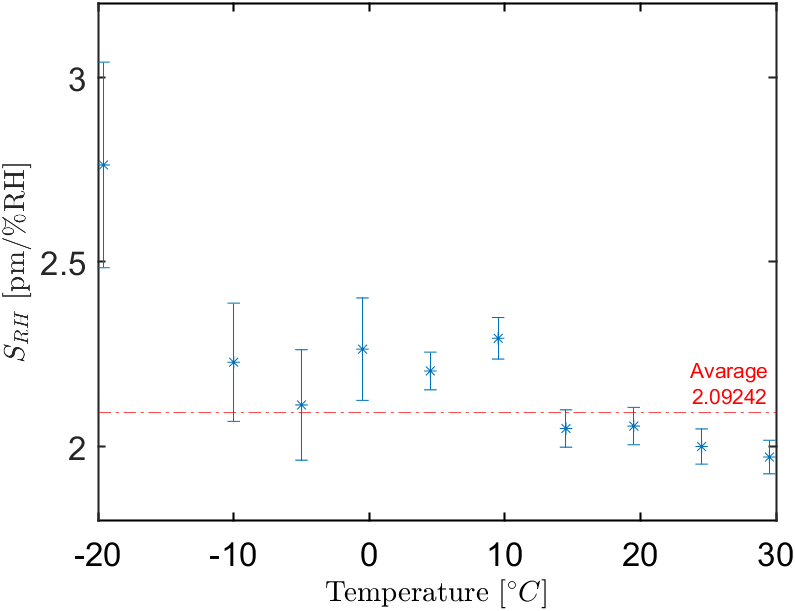
\includegraphics[width=0.55\columnwidth]{Chapter5/images/RHS_RH.png}
\caption{Humidity sensitivity ($S_{RH}$ at different temperatures with the corresponding uncertainty for the FBG-based hygrometer.}
\label{fig_RH_sens}
\end{figure}
\begin{figure}[!h]
\centering
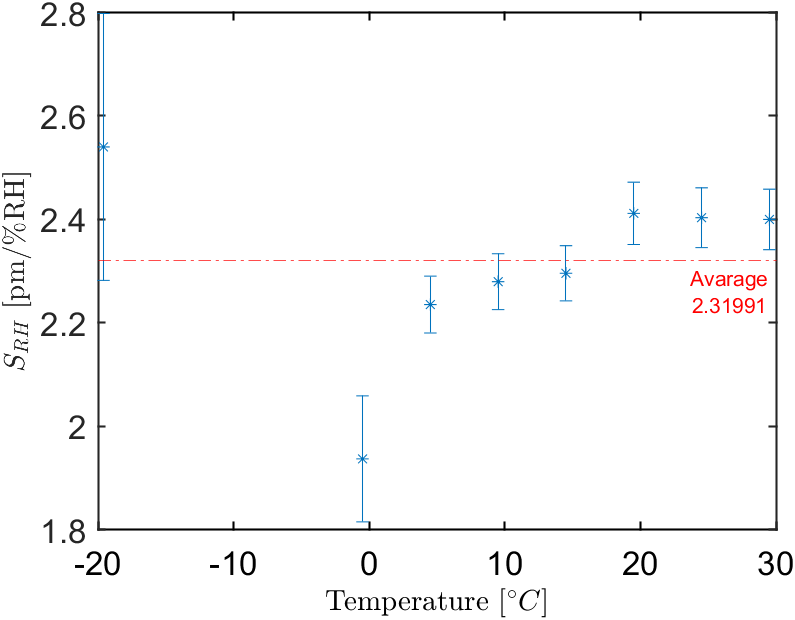
\includegraphics[width=0.55\columnwidth]{Chapter5/images/RH1_RH.png}
\caption{Humidity sensitivity $S_{RH}$ at different temperatures with the corresponding uncertainty for the first \gls{RH} sensor in the array.}
\label{fig_RH_sens2}
\end{figure}

Similar plots were also obtained for all the other \gls{RH} sensors of the array (see Figure~\ref{fig_calibration}). The second hygrometer didn't show a linear response to the changing conditions, which is further discussed in the next section.
\newpage
The average $S_{RH}$ for the array sensors is $2.77\pm 0.03~\mathrm{\frac{pm}{\%RH}}$  and $2.09\pm 0.02~\mathrm{\frac{pm}{\%RH}}$ for the hygrometer. Given the uncertainty of the coating thickness, these results are in line with the findings in~\cite{YEO_PI} and~\cite{Kronenberg:02} for coating thicknesses between \SI{15}{\micro\metre} and \SI{20}{\micro\metre}. The uncertainty obtained from the calibration is much smaller than the error introduced by the interrogator itself, which is $1$~pm. The hygrometer measures with an accuracy of 0.5~\%RH and for the array sensors on average 0.36~\%RH. 

\begin{figure}[!h]
\centering
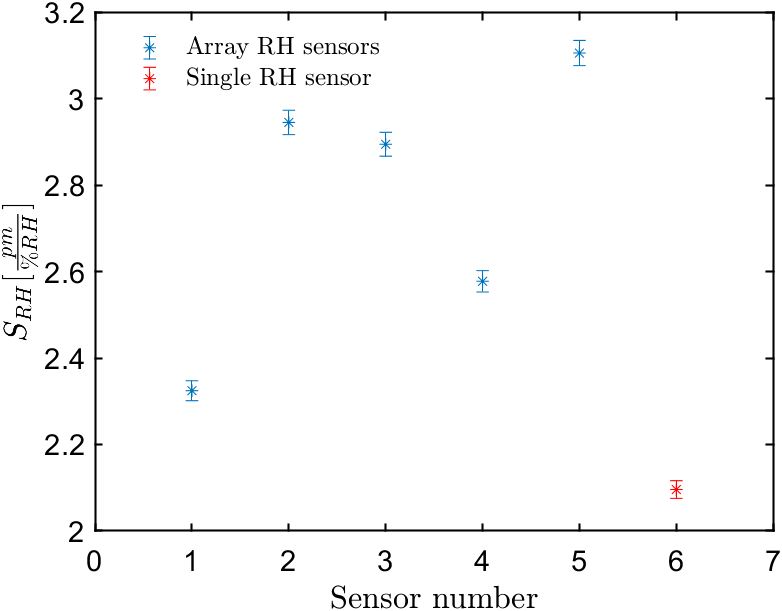
\includegraphics[width=0.57\columnwidth]{Chapter5/images/comp1.png}
\caption{Humidity sensitivity $S_{RH}$ of the sensors with the corresponding uncertainty.}
\label{fig_calibration}
\end{figure}
\newpage
The second coefficient called temperature sensitivity ($S_{T}$) conveys information on how the wavelength shifts depends on the changing temperature. In this case, for the stable \gls{RH} values, the temperature was changed between \SI{-20}{\celsius} and \SI{30}{\celsius}. The average temperature sensitivity $S_{T}$ value for the array is $10.25\pm0.02\,\mathrm{\frac{pm}{^{\circ}C}}$ and for the hygrometer $10.87\pm 0.02\,\mathrm{\frac{pm}{^{\circ}C}}$ (see Figure~\ref{fig_calibration1}). The $S_{T}$ is about an order of magnitude larger than the humidity sensitivity ($S_{RH}$). That implies that the temperature sensor located next to the \gls{RH} one should measure with good accuracy, in order to avoid a huge uncertainty of the humidity measurement. A \SI{0.1}{\celsius} temperature uncertainty leads to almost $0.5$\%RH uncertainty in the case of the hygrometer and $0.36$\%RH in the \gls{RH} array. 

\begin{figure}[!h]
\centering
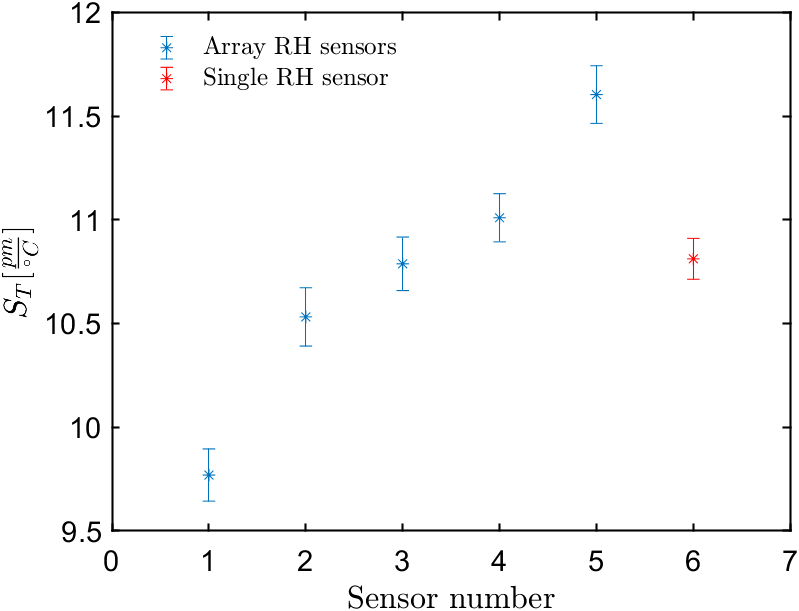
\includegraphics[width=0.57\columnwidth]{Chapter5/images/comp.png}
\caption{Temperature sensitivity $S_{T}$ of the sensors with the corresponding uncertainty.}
\label{fig_calibration1}
\end{figure}

\subsection{Calibration with saturated salt solutions}
The two mentioned hygrometers were also at first tested with the use of the saturated salt solutions method. The details of this approach are given in section~\ref{fos:setup}. The results of these measurements are depicted in Figure~\ref{fig:fos_salt}. The Sensor depicted as FBG RH FOS 1 doesn't have a linear response to the changing humidity and temperature, therefore it was excluded from further tests. 

\begin{figure}[!h]
\centering
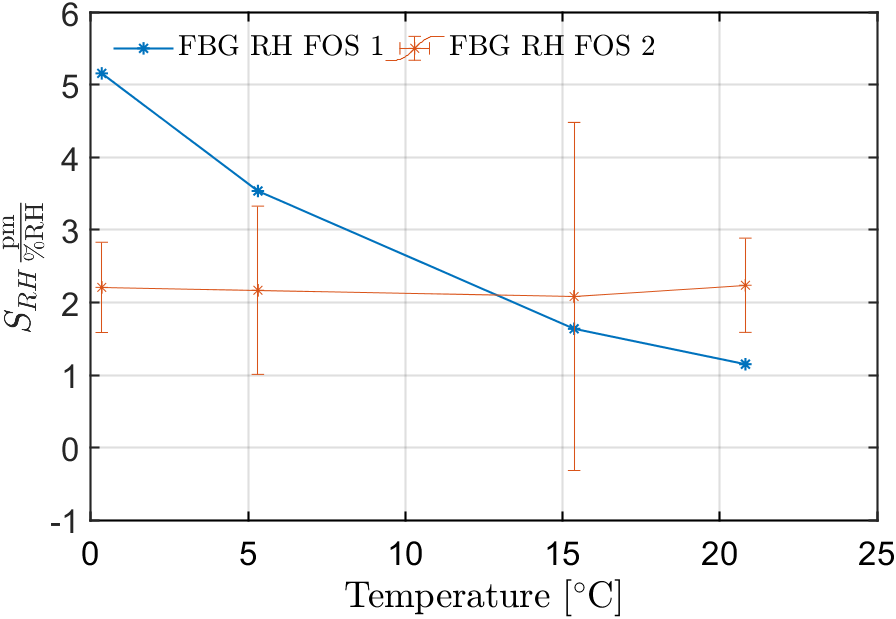
\includegraphics[width=0.48\columnwidth]{Chapter5/images/salt_srh.png}
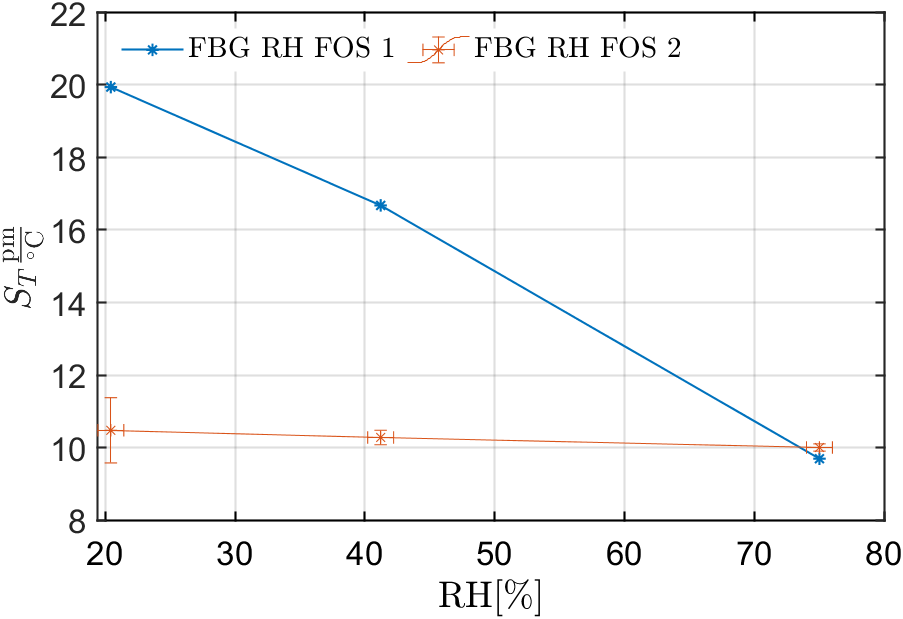
\includegraphics[width=0.49\columnwidth]{Chapter5/images/salt_st.png}
\caption{Relative humidity $S_{RH}$ and temperature sensitivity $S_{T}$ as per the results from the calibration with the saturated salt solutions. Average error for the $S_{RH} = \pm $\SI{1.21}{\pico\metre} and for the $S_{T}=\pm$ \SI{0.4}{\pico\metre}.}
\label{fig:fos_salt}
\end{figure}

The comparison of the results from two different calibration methods for the hygrometers is depicted in Table~\ref{tab:fos}. The calibration method based on the saturated salt solutions has larger uncertainties due to the small number of calibration points. Nevertheless, the method involving saturated salt solutions is a very cost-effective method allowing the characterization of the sensors, but it can't be used in a wide temperature range, especially below \SI{0}{\celsius} as the relative humidity provided by the solution is not constant. 

% Please add the following required packages to your document preamble:
% \usepackage{graphicx}
% Please add the following required packages to your document preamble:
% \usepackage{graphicx}
\begin{table}[!h]
\centering
\caption{Comparison of the temperature and humidity sensitivity obtained through calibration based on different approaches.}
\label{tab:fos}
\resizebox{\textwidth}{!}{%
\begin{tabular}{lcccc}
Means of controlling humidity & $S_{RH} \mathrm{[\frac{pm}{\%RH}]}$ & \multicolumn{1}{l}{$S_{RH}$ uncertainty {[}pm{]}} & $S_{T}\mathrm{[\frac{pm}{\SI{}{\celsius}}}]$ & \multicolumn{1}{l}{$S_{T}$ uncertainty {[}pm{]}} \\ \hline
Saturated salt                & 2.17                                & 1.21                                              & 10.25                                        & 0.4                                              \\
Climatic chamber              & 2.09                                & 0.06                                              & 10.87                                        & 0.02                                            
\end{tabular}%
}
\end{table}
\subsection{Time response}
The time response of the hygrometer and the array sensors was investigated as well. The sensors were compared during the increasing humidity from about 20\% to 80\%. The \gls{FBG} based \gls{FOS} has a much longer time response than the capacitive sensors (seconds). The time response of different sensors is often compared using for example the time to reach 63\% of set value $\tau_{63}$.
\newpage
Figures~\ref{fig_time_response} and~\ref{fig_time_response2} depict the comparison of the time response of the hygrometer and one of the array sensors with commercial capacitive sensors (two SHT85 and HYT221 sensors). The response of the \gls{FOS} is shown as wavelength change. It's also noteworthy that the response is about twice slower at \SI{0}{\celsius}. The average response time at \SI{0}{\celsius} for the array sensors is $10.7$~min, and $4.8$~min for the hygrometer. On the other hand, at \SI{20}{\celsius} those values equal $2.3$~min and $2$~min. Small differences among the array sensors were also seen, but they most likely correspond to slight differences in the coating thickness and the position inside the climatic chamber. 

\begin{figure}[!h]
\centering
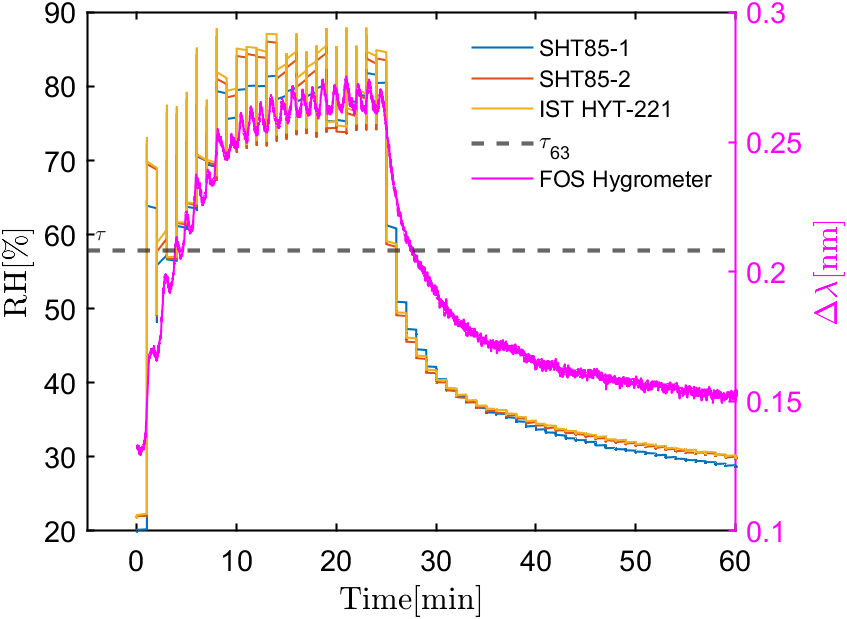
\includegraphics[width=0.47\columnwidth]{Chapter5/images/20responseRH.png}
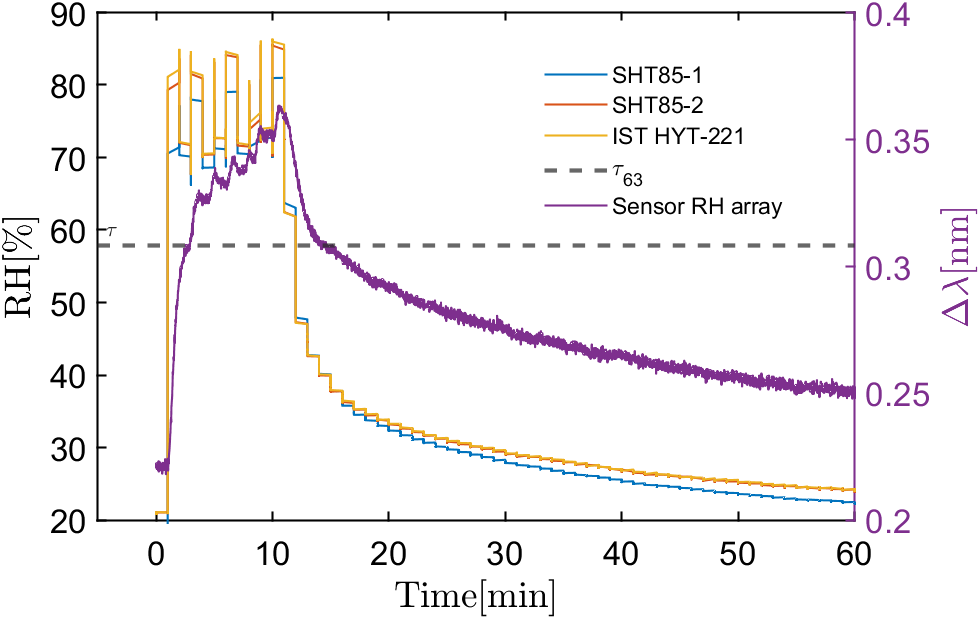
\includegraphics[width=0.47\columnwidth]{Chapter5/images/20responseRH2.png}
\caption{Time response of the hygrometer and array sensors, and comparison to the capacitive sensors. The dashed line represents the 63\% of the final \gls{RH} value at \SI{0}{\celsius}.}
\label{fig_time_response}
\end{figure}

\begin{figure}[!h]
\centering
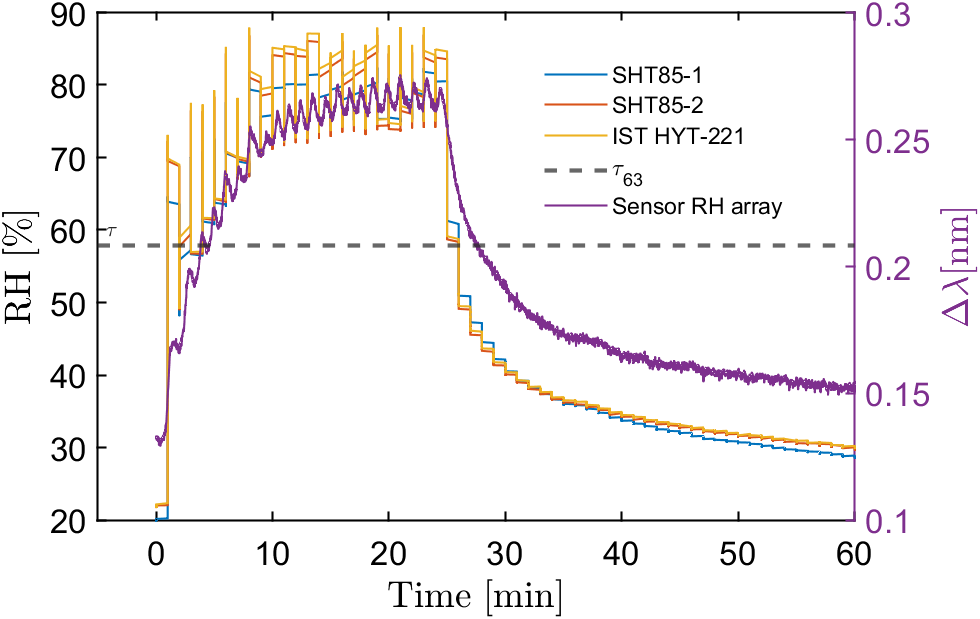
\includegraphics[width=0.47\columnwidth]{Chapter5/images/020responseRH.png}
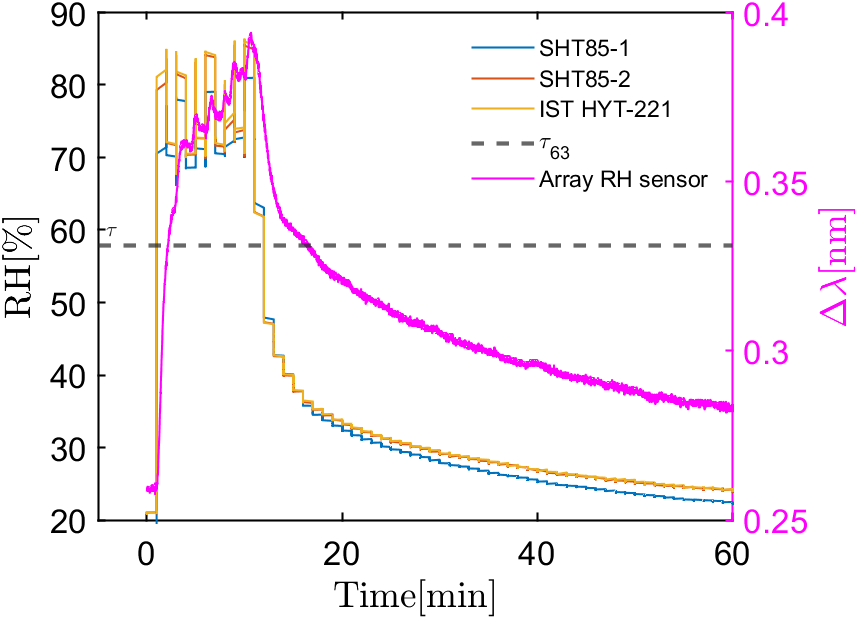
\includegraphics[width=0.47\columnwidth]{Chapter5/images/020responseRH2.png}
\caption{Time response of the hygrometer and array sensors, and comparison to the capacitive sensors. The dashed line represents the 63\% of the final \gls{RH} value at \SI{20}{\celsius}.}
\label{fig_time_response2}
\end{figure}

Longer response times for the array sensors are related to the thicker polyimide coating. The second contribution might be related to the slightly different packaging of the sensors. 

\subsection{Hysteresis}
Figures~\ref{fig_hysteresis} and~\ref{fig_hysteresis2} show the hysteresis of the hygrometer and two array sensors. The first figure shows the wavelength change during the stepwise increase of relative humidity from $10$\% to $70$\% (with $10$\% step), and also while decreasing the \gls{RH}. The temperature fluctuations during the hysteresis measurement are depicted in Figure~\ref{fig_hysteresis2}. The resolution of the optical interrogator is $1$~pm. Hence, any temperature uncertainty of \SI{0.1}{\celsius} and relative humidity uncertainty of $0.5$\% are related to the device resolution. Based on Bragg wavelength measurement differences at each point, the hysteresis of the hygrometer is $0.72\pm0.48$\%RH and for the array sensors $2.67\pm0.33$\%RH. 

\begin{figure}[!h]
\centering
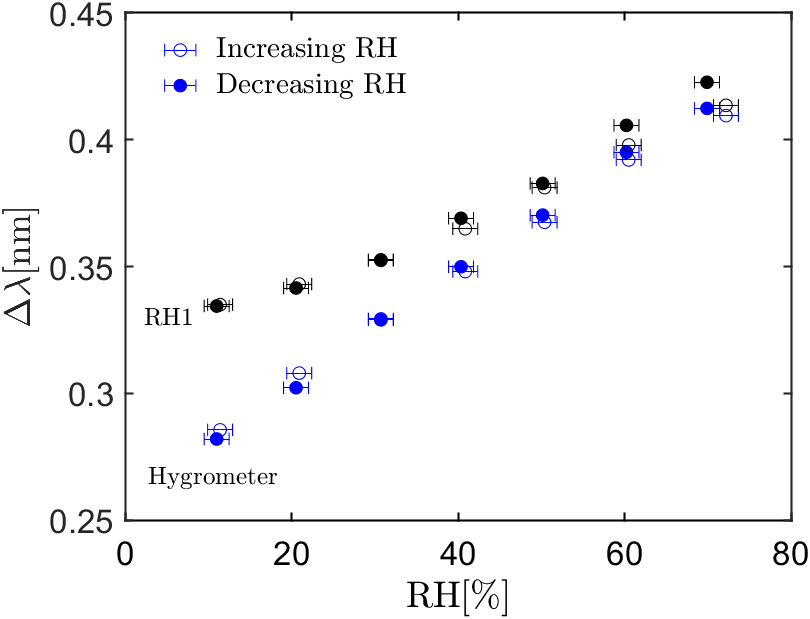
\includegraphics[width=0.57\columnwidth]{Chapter5/images/25_RHS.png}
\caption{Hysteresis of the hygrometer and the first array sensor at a constant temperature of \SI{25}{\celsius}.}
\label{fig_hysteresis}
\end{figure}

\begin{figure}[!h]
\centering
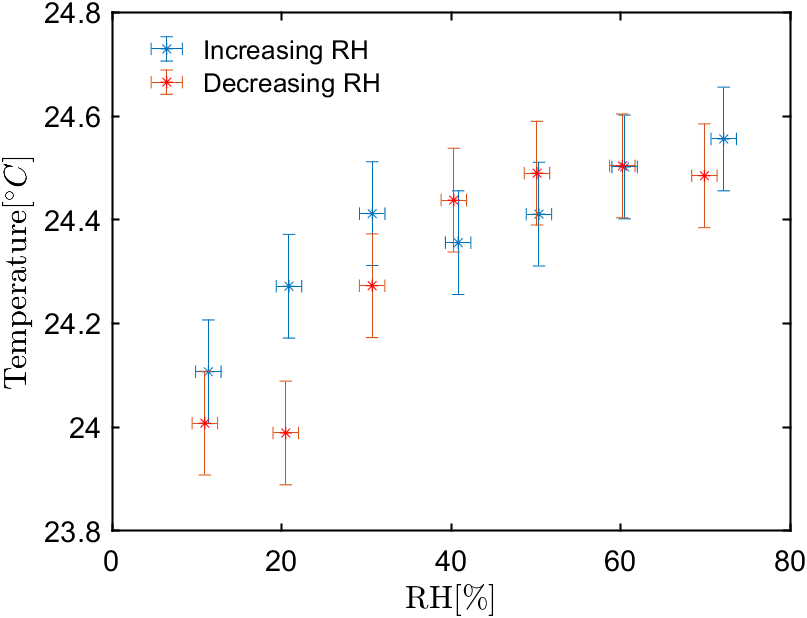
\includegraphics[width=0.57\columnwidth]{Chapter5/images/25_RHST.png}
\caption{Temperature stability during the hysteresis measurement.}
\label{fig_hysteresis2}
\end{figure}
\newpage
\subsection{Repeatability}
The repeatability of the hygrometer was also determined by performing three measurements that involved increasing humidity from about $10$\% to $80$\% and then decreasing it again in steps of $10$\% to the baseline value. The sensor shows acceptable stability and repeatability after 7 days since the first measurement. The sensors in the array showed a large offset which is most likely related to the holder/packaging of the sensor and the difficulty to keep the sensors in strain-free conditions, as they are located very close to each other (less than $15$~cm).
\begin{figure}[!h]
\centering
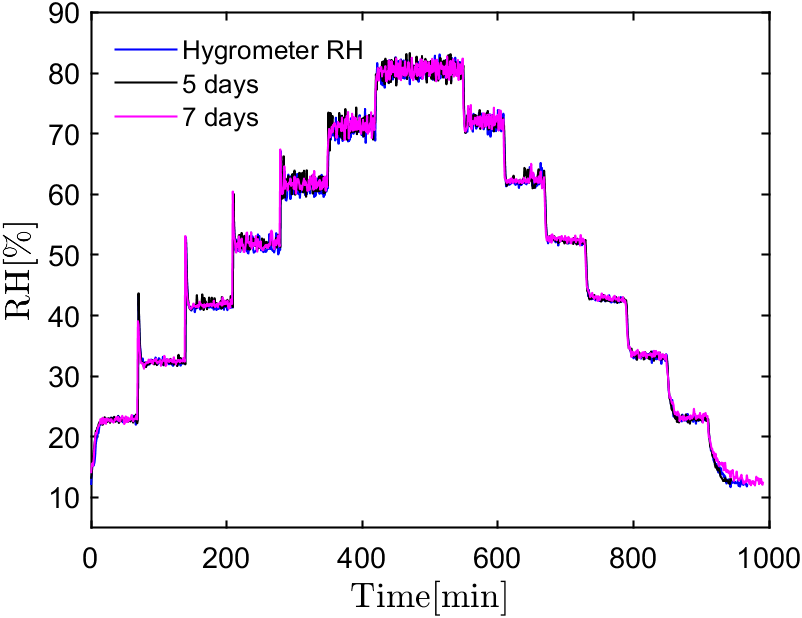
\includegraphics[width=0.6\columnwidth]{Chapter5/images/repeat.png}
\caption{Repeatability of the hygrometer. Three subsequent measurements were compared after 5 and 7 days after the first test.}
\label{fig_repeatability}
\end{figure}




